% !TEX root = ../notes_missingsemester.tex
% Chapter 1: Servers, VMs and Linux Basics
%%%%%%%%%%%%%%%%%%%%%%%%%%%%%%%%%%%%%%%%%%%%%%%%%%%%%%%%%%%%%%%%%%%%%%

% POST IMPROVEMENTS 2026:
% 3. Offer a preconfigured OVA for students who cannot complete VM install in session.
% 4. Offer a preconfigured version for Gnome and UTM users, with instructions for importing and network setup.



\index{Virtual Machines}\index{Linux}\index{SSH}\index{Oracle VirtualBox Manager}
\chapter{Development and Production}
\printchapterversion{01_servers_vms_linux}
\newthought{Divide and conquer.}

% ==============================================================================================
% BLOCK 1: INTRODUCTION
% ==============================================================================================

\section{The Why}\index{server}\index{dev VM}

Most software engineering curricula focus on algorithms, data structures, and the theory of computation.
Writing a Python script that runs once on a single laptop is a skill; making that script available as a service,
keeping it running, and recovering when it fails is a different one.
This course addresses the second set of skills, the tools and workflows
that sit between working code and the full stack of setting up and maintaining a running system. 


\marginnote{\newthought{PixelWise} is the narrative thread of the entire course.
Users draw a digit on a pixelated $28{\times}28$ canvas in the browser,
the backend runs an image classifier trained on MNIST\index{MNIST},
the model predicts class and confidence, and results are stored in a database.}

\newthought{Across ten lecture blocks we build PixelWise}\index{PixelWise},
a handwritten digit recognition web application.
The starting point is two empty virtual machines; the end point is a deployed service including a frontend, 
and a backend with a trained model, an API, 
and a database, all running on Linux servers and connected over a network,
with version control, automated deployment, persistent storage, and monitoring.
Each tool we introduce is motivated by a specific need that arises in the construction of a fullstack application: Pixelwise.

\marginnote{\newthought{This enables you} to deploy your own prooducts and services in the future.}



\newthought{Development and Production.}

\begin{figure}
\centering
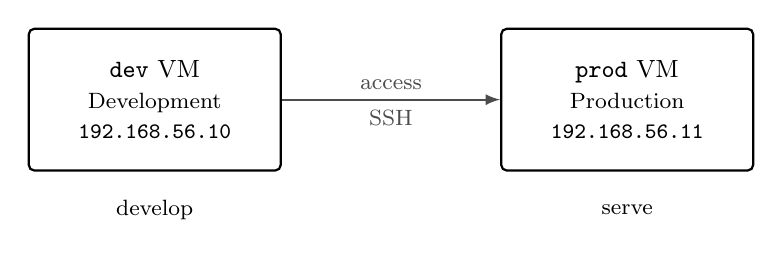
\begin{tikzpicture}[
    every node/.style={font=\small, align=center},
    vm/.style={rectangle, draw=black, thick, rounded corners=2pt, minimum width=3.2cm, minimum height=1.8cm, inner sep=6pt},
    arr/.style={-latex, thick, black!70}
]
% Dev VM (left)
\node[vm] (dev) at (0, 0) {\texttt{dev} VM\\\footnotesize Development\\\footnotesize \texttt{192.168.56.10}};
\node[font=\footnotesize] at (0, -1.4) {develop};

% Prod VM (right)
\node[vm] (server) at (6, 0) {\texttt{prod} VM\\\footnotesize Production\\\footnotesize \texttt{192.168.56.11}};
\node[font=\footnotesize] at (6, -1.4) {serve};

% Arrow between them
\draw[arr] (dev.east) -- node[above, font=\footnotesize] {access} node[below, font=\footnotesize] {SSH} (server.west);
\end{tikzpicture}
\caption{The two-machine setup. The dev VM is where code is written and tested; the prod VM is where the deployed application runs. Code travels from dev to prod through a deliberate deployment step over SSH.}
\label{fig:two_machines}
\end{figure}

The figure shows the starting arrangement: two virtual machines
that play distinct roles throughout the course.
The \texttt{dev} VM is the development environment in which code is written, modified, and tested.
The \texttt{prod} VM is the production environment in which the deployed application runs.
Later blocks add the backend stack, the frontend, persistence, and automation between the two,
but the separation between development and production stays intact from this block onward.






\iffalse
\newthought{The final project structure} is our map from day one.
Each folder is empty until the block that introduces it, but the shape is here now,
so you always know where things are headed.

\begin{verbatim}
pixelwise/
+-- app/                  # B3 -- Python package (backend)
|   +-- __init__.py
|   +-- main.py           # B5 -- FastAPI app
|   +-- models.py         # B6 -- SQLAlchemy models
|   +-- classifier.py     # B4 -- model inference wrapper
+-- data/                 # B4 -- training data, gitignored
+-- models/               # B4 -- trained model artefacts, gitignored
+-- frontend/             # B7 -- HTML/CSS/JS drawing canvas
+-- nginx/                # B7 -- Nginx config
+-- scripts/              # B8 -- deploy, backup scripts
+-- tests/                # B8 -- CI test suite
+-- train.py              # B4 -- reproducible training script
+-- predict.py            # B4 -- CLI inference, replaced by API in B5
+-- requirements.txt      # B3 -- pinned dependencies
+-- .env.example          # B3 -- grows block by block
+-- .gitignore
+-- README.md
\end{verbatim}


\marginnote{\newthought{Reading the tree} alongside the figure,
\texttt{app/} and \texttt{nginx/} produce the backend stack on \texttt{prod},
\texttt{frontend/} produces what the browser renders,
and \texttt{scripts/} is the bridge that carries code from \texttt{dev} to \texttt{prod}.
Every folder maps to a role in Figure~\ref{fig:two_machines}.}
\fi

\subsection{Hands On Experience}

\newthought{Consider a small web application} running on your laptop.
A classmate two time zones away wants to try it; you send them the address.
It works, until you close the lid to catch a train.
That evening the Wi-Fi has changed, the address is different,
and the process you started in the terminal is gone.

\marginnote{\newthought{Count the hours} your laptop is actually reachable at a stable address.
Subtract the time it is closed, asleep, on battery, behind a caf\'e router, or rebooting after an update.
What remains is the service level a laptop alone can offer.}

\newthought{A server} is a machine whose job is to be available when no one is watching.
It stays powered on, holds a stable address, and answers requests around the clock.
Your laptop is where code is written and changed; the server is where code meets users.
Keeping these two roles on separate machines is the first design decision of the course.

\marginnote{\newthought{Two machines, one mental model.}
\texttt{dev} at $192.168.56.10$ stands in for your laptop.
\texttt{prod} at $192.168.56.11$ stands in for the always-on host.
Later lectures fill in the bridge.}

\newthought{This first block} focuses on machines and environments rather than on code.
Before introducing a programming language, a version control system, or a framework,
we need a place which is always up, to run programs, isolated from experiments, and a place for development.
By the end of the block you will have provisioned both virtual machines,
\begin{itemize}
    \item set up a server and a development machine as virtual machines on your laptop,
    \item learned the subset of Linux needed to navigate a server from the command line,
    \item and configured remote access over SSH using key-based authentication.
\end{itemize}




% ==============================================================================================
% BLOCK 2: CONCEPTS AND PRACTICE
% ==============================================================================================

\newpage
\section{Virtual Machines}\index{Virtual Machines}\index{hypervisor}

\newthought{A virtual machine is a simulated computer} running inside your real computer.
The software that creates and runs virtual machines is called a hypervisor.
The hypervisor partitions the host's CPU, memory, and disk, and presents each virtual machine
with what appears to be its own hardware.
From the guest operating system's perspective, it is running on a physical machine.

\newthought{Hypervisors} are often categorised as type~1 or type~2.
A type~1\index{type-1 hypervisor} hypervisor runs directly on the hardware,
with the host operating system built into the hypervisor itself.
Examples include VMWare ESXi and Microsoft Hyper-V in its server role;
cloud providers use type~1 hypervisors to host the virtual machines you rent.
A type~2\index{type-2 hypervisor} hypervisor runs as an application on top of a regular operating system.
Oracle VirtualBox Manager is a type~2 hypervisor, which is why we can install it as a normal program
on Windows, macOS, or Linux.
The conceptual model is the same in both cases; the differences are in performance and deployment context.

\newthought{Isolation} is the primary reason to use a virtual machine.
A misconfiguration, an uninstalled package, or a destructive command inside the guest
does not affect the host operating system.
Because the hypervisor abstracts away the hardware, the same VM runs identically on Windows, macOS, and Linux hosts,
which is the basis of the reproducibility argument.

\marginnote{\newthought{A snapshot}\index{snapshot} captures the entire machine state at a point in time,
including disk contents, memory, and running processes.
Snapshots are inexpensive to create and well-suited to exploratory work;
making one before a risky change and restoring it afterwards is a standard pattern.}

\newthought{There are costs.}
A virtual machine executes a full operating system on top of the host,
which carries a performance overhead that is typically small for I/O-bound work and larger for CPU-bound work.
Each VM reserves some amount of RAM, disk space, and CPU time from the host,
so the number of concurrent VMs is limited by available resources.
Boot time is longer than launching an application but shorter than booting physical hardware.
These costs are the price paid for isolation, reproducibility, and rollback.

\marginnote{\newthought{Outside the classroom,}
a production host is usually a rented or purchased server in a data centre,
and the development machine is the laptop or workstation in front of you.
Running both as VMs inside a single laptop is a teaching shortcut:
it preserves the two-machine separation without asking you to rent hardware,
and everything we learn here transfers directly when \texttt{prod} is later replaced
by a cloud instance reached over the public internet.}

\newthought{Host-only networking} puts \texttt{dev} and \texttt{prod} on a private subnet,
typically $192.168.56.0/24$, that only the host and the guests can reach.
The guests get internet through a second, NAT-mode adapter,
so they can install packages without being exposed to the outside world.
We assign static IPs, $192.168.56.10$ for \texttt{dev} and $192.168.56.11$ for \texttt{prod},
so that every command in the course refers to the same addresses.











% ==============================================================================================
\newpage
\section{Exercise: Provisioning Virtual Machines}\index{exercises}

\marginnote{\newthought{Exercises} are for practice and reinforcing concepts.
Work through them yourself first, break things, discuss, this is not a time trial.
If your VM ends up in a state you cannot recover, restore the \texttt{B1-fresh} snapshot and start over.
At the end of the session, take a snapshot named \texttt{B1-complete}, your safety net for the next block.}


\newthought{Install the Oracle VirtualBox Manager} for your host OS with default settings, and download two Ubuntu LTS ISOs (go for version 24.x.x if you find one): the Desktop edition for \texttt{dev} and the Server edition for \texttt{prod}. The asymmetry is deliberate, \texttt{dev} carries a graphical environment so you can run an editor and a browser locally, while \texttt{prod} stays headless because a production server has no business running a desktop.
You can also decide to run dev on your machine directly, but this is not further supported in the excercises.

\marginnote{\newthought{Where to get them.} VirtualBox: \url{https://www.oracle.com/virtualization/virtualbox/}. 
Ubuntu Desktop LTS ISO: \url{https://ubuntu.com/download/desktop}. Ubuntu Server LTS ISO: \url{https://ubuntu.com/download/server}. 
Pick the LTS release in both cases, not the interim one, so support extends across the semester. 
On an Ubuntu host you can use GNOME Boxes instead: \url{https://apps.gnome.org/Boxes/}. O
n macOS, UTM is the closest equivalent: \url{https://mac.getutm.app/}.}


\marginnote{\newthought{Installer choices} that matter: use distinct credentials per VM, \texttt{user}/\texttt{password} on \texttt{dev} and \texttt{produser}/\texttt{prodpassword} on \texttt{prod}. The asymmetry is deliberate, you should feel that logging into \texttt{prod} is a different act from working on \texttt{dev}.}

\newthought{Create the \texttt{dev} VM} in the Oracle VirtualBox Manager. Click \texttt{New} and configure:
\begin{itemize}
    \item Name \texttt{dev}, Type \texttt{Linux}, Version \texttt{Ubuntu (64-bit)}
    \item Memory at least 4096\,MB, CPUs at least 2
    \item Hard disk at least 25\,GB, VDI, dynamically allocated
\end{itemize}


\newthought{Create the \texttt{prod} VM} with the same procedure but tighter resources, since it runs headless:
\begin{itemize}
    \item Name \texttt{prod}, Type \texttt{Linux}, Version \texttt{Ubuntu (64-bit)}
    \item Memory at least 2048\,MB, CPUs at least 2
    \item Hard disk at least 10\,GB, VDI, dynamically allocated
\end{itemize}

\marginnote{\newthought{Why the spread.} Ubuntu Desktop with GNOME wants roughly 4\,GB of RAM and 25\,GB of disk to feel responsive. Ubuntu Server has no GUI and runs comfortably in a quarter of that. Sized this way the pair fits inside a 6\,GB / 35\,GB envelope on the host.}

\newthought{Attach the matching ISO} to each VM. VirtualBox offers an unattended installation checkbox during creation, don't select it, 
you want the interactive installer. Once a VM exists, select it in the manager and open \texttt{Settings}, \texttt{Storage}. Under \texttt{Storage Devices} you will see a controller, \texttt{IDE} or \texttt{SATA}, with an \texttt{Empty} optical drive beneath it. Click that \texttt{Empty} entry, then on the right under \texttt{Attributes} click the small disc icon next to \texttt{Optical Drive}, choose \texttt{Choose a disk file}, and pick the Desktop ISO for \texttt{dev} or the Server ISO for \texttt{prod}. Confirm with \texttt{OK}, start the VM, follow the installer, when in doubt go with the defaults and just forward-enter.


\newthought{After the first boot of each VM (both dev and prod), install the OpenSSH server to enable remote access:}
\begin{verbatim}
sudo apt update
sudo apt install openssh-server
\end{verbatim}
This step is required for both Desktop and Server editions. Reboot after installation.

\marginnote{\newthought{German keyboard?}\index{keyboard layout}
The interactive installer often defaults to a US layout, which turns
every hunt for a slash, tilde, or brace into a guessing game. Switch
to German with:\\[0.4em]
\texttt{sudo dpkg-reconfigure keyboard-configuration}\\[0.3em]
Pick \texttt{Generic 105-key} when prompted, then \texttt{German},
and accept the defaults for the rest.}


\marginnote{\newthought{Host-only network.} In \texttt{File}, \texttt{Host Network Manager} (or \texttt{File}, \texttt{Tools}, \texttt{Network Manager} on version~7+), create a host-only network if none exists, typically $192.168.56.1/24$.

\vspace{0.4em}
\newthought{Disable DHCP} on this network so the static IPs you assign by hand in the next step are not overwritten.}

\newthought{Configure the network adapters for each VM:}
Select the VM in VirtualBox Manager and open \texttt{Settings}, then go to the \texttt{Network} section. 
For Adapter~1, check "Enable Network Adapter" and set it to \texttt{NAT} (for internet access). 
For Adapter~2, select the Adapter~2 tab, check "Enable Network Adapter," set it to \texttt{Host-only Adapter}, 
and choose the host-only network you created.

\marginnote{\newthought{Missing Adapter~2?} Power-off the VM, make sure you are in Expertmode, go to \texttt{Settings}, \texttt{Network}, select Adapter~2, check "Enable Network Adapter," and set it to \texttt{Host-only Adapter}.}


\newthought{Assign static IPs inside each VM:}
\marginnote{\newthought{Open a terminal (Desktop).} On Ubuntu Desktop press \texttt{Ctrl+Alt+T}, or open \texttt{Activities} (top-left) and type ``terminal''; press Enter. You can also right-click the desktop and select "Open Terminal" if the menu is present.}
\begin{enumerate}
    \item Boot the VM and log in.
    \item Run \texttt{ip a} to list network interfaces. The host-only adapter is usually \texttt{enp0s8}, but confirm whether the name shows up in the output.
    \item Edit the Netplan config with \\
    \texttt{sudo nano /etc/netplan/00-installer-config.yaml}
    Save and exit nano with ( Ctrl+X, Y, Enter).
    \item For \texttt{dev}, set the config as:

    \marginnote{For \texttt{prod}, use \texttt{192.168.56.11/24} instead.}
\begin{verbatim}
network:
  version: 2
  ethernets:
    enp0s8:
      addresses:
        - 192.168.56.10/24
\end{verbatim}

    \item Apply the config with \texttt{sudo netplan apply}
    \marginnote{\newthought{Netplan permission warning.} Netplan will warn if a configuration file is writable by group/others or not owned by \texttt{root}. This is a security check to avoid loading untrusted configuration files; expected ownership is \texttt{root:root} and modes such as \texttt{644} for the YAML files.}
    \item Check the new address with \texttt{ip a} again; you should see the static IP assigned to \texttt{enp0s8}.
\end{enumerate}

\marginnote{\newthought{Troubleshooting.} If the interface name is not \texttt{enp0s8}, use the correct one from \texttt{ip a}.}


\newthought{Verify connectivity:}
On \texttt{dev}, run \texttt{ping 192.168.56.11} to test if \texttt{prod} responds. If you get no reply, double-check the Netplan configuration (correct interface and address), ensure Adapter~2 is set to Host-only in both VMs, and confirm that both VMs are running and attached to the same host-only network.
\begin{figure}[ht]
    \centering
    \includegraphics[width=1\linewidth]{./figures/vm_ping.png}
    \caption{ping}
    \label{fig:vm_ping}
\end{figure}








% ==============================================================================================
\newpage
\section{Linux on the Server}\index{Linux}\index{Ubuntu}

\newthought{Linux} is a family of Unix-like operating systems built around a common kernel,
first released by Linus Torvalds in 1991.
A distribution\index{distribution} combines the kernel with a package manager,
system libraries, and user-space tools into a coherent product.
Ubuntu\index{Ubuntu}, Debian, Fedora, and Arch are distributions that differ in release cadence and defaults
but share most of what matters at the command line.

\marginnote{\newthought{Ubuntu}\index{Ubuntu} at \url{https://ubuntu.com/} is the distribution we use on both VMs.
Long-term support releases receive five years of security updates,
which is why we pick the LTS ISO rather than the latest release.}

\begin{marginfigure}
    \centering
    \includegraphics[width=\marginparwidth]{./figures/vm_running.png}
    \caption{A running Ubuntu guest inside the Oracle VirtualBox Manager. The guest believes it owns a physical machine; the hypervisor is what makes that illusion hold.}
    \label{fig:vm_running}
\end{marginfigure}

\newthought{A server in this section} is a computer configured to run services and accept connections over a network,
typically without a graphical session.
You interact with it through a shell, a program that reads commands and prints their output;
the shell we use is Bash\index{Bash}, the default on Ubuntu.



\marginnote{\newthought{The Unix philosophy}\index{Unix philosophy} shapes the design of these tools.
Each program does one thing well, programs pass streams of text to each other, and configuration lives in plain files.
The result is a small vocabulary of composable commands that combine into pipelines no single command was designed for.}

\newthought{Five commands} are sufficient for the first session.
\texttt{ls} lists a directory, with \texttt{-la} showing permissions, ownership, and hidden files.
\texttt{cd} changes directory; \texttt{cd ..} moves up one level and \texttt{cd \~{}} returns home.
\texttt{pwd} prints the current path, \texttt{mkdir} creates a directory,
and \texttt{cat} prints a file to the terminal.

\vspace{2.5em}
\newthought{Linux is a multi-user operating system.}
Every file belongs to a user and a group and carries three permission sets, for owner, group, and everyone else.
Each set independently grants read, write, or execute access.
\texttt{whoami}\index{whoami} reports the current user, and \texttt{ls -la} shows ownership and permissions:

\begin{verbatim}
-rw-r--r-- 1 user user 1234 Jan 15 10:00 config.txt
drwxr-xr-x 2 user user 4096 Jan 15 10:00 mydir/
\end{verbatim}

\marginnote{\newthought{Reading the mode string} from left to right,
the first character tells you whether it is a file or directory,
then three groups of \texttt{rwx} for owner, group, others.
A dash means the permission is not granted. The leading \texttt{d} marks a directory.}

\newthought{Two commands} modify these.
\texttt{chmod}\index{chmod} changes permissions and \texttt{chown}\index{chown} changes ownership:

\begin{verbatim}
chmod 600 ~/.ssh/id_ed25519           # owner-only read and write
sudo chown user:user file.txt         # assign user and group
\end{verbatim}

The principle of least privilege\index{least privilege} applies throughout the course:
grant each user, process, or service only the access it needs,
so that narrow defaults limit the blast radius of a compromise or a mistake.




% ==============================================================================================
\newpage
\section{Exercise: Navigating Linux}\index{exercises}
\marginnote{\newthought{Ten-finger typing}\index{touch typing} is part of the toolchain once the terminal is your main tool.
A server has no menus, so your throughput is bounded by how quickly you can speak to the shell without looking at the keys;
every hunt for a slash, tilde, or brace is attention spent on the keyboard instead of the problem.
Ten minutes a day at \url{https://www.keybr.com/}, \url{https://typing.io/}, or \url{https://monkeytype.com/}
is enough to remove that tax over a few weeks.}

\newthought{This exercise} turns the five commands and the permission model into something your hands remember. You walk the directories common to every Linux system, identify yourself to the machine, and read and change a file's mode string. By the end, the output of \texttt{ls -la} should read as a description you can speak aloud rather than a blob of symbols.

\newthought{Explore the filesystem} by visiting \texttt{/home}, \texttt{/etc}, and \texttt{/opt} in turn with \texttt{cd} and \texttt{ls -la}, and read two files with \texttt{cat}:

\begin{verbatim}
cat /etc/hostname
cat /etc/os-release
\end{verbatim}

\marginnote{\newthought{The filesystem as map.}
\texttt{/home} is where users live, \texttt{/etc}\index{/etc} holds configuration, and \texttt{/opt}\index{/opt} is where PixelWise will be installed in a later block.
These locations reflect decades of convention you will meet on every Linux machine; knowing them lets you locate things by instinct.}

\newthought{Create a workspace} and check that you are where you think you are:

\begin{verbatim}
mkdir ~/workshop && cd ~/workshop
pwd
touch notes.txt
rm notes.txt
\end{verbatim}

\texttt{pwd} is a reassurance command. When something does not behave as you expect, asking the shell where it thinks it is usually explains the problem faster than re-reading the error.

\newthought{Understand who you are} and look at the permissions on your new file:

\begin{verbatim}
whoami
id
ls -la notes.txt
\end{verbatim}

Decode the first column of \texttt{ls -la} against the margin note on mode strings from the theory above. Name aloud what each of the ten characters means; if you can do that without looking, permissions have stopped being mysterious.

\newthought{Change the mode and watch it:}

\begin{verbatim}
chmod 600 notes.txt
ls -la notes.txt
\end{verbatim}

\marginnote{\newthought{A thought experiment on least privilege.}
Your \texttt{user} account can read \texttt{/etc/os-release} but cannot edit \texttt{/etc/ssh/sshd\_config} without \texttt{sudo}. Why does that separation exist, and what would change if the web service we deploy in a later block ran as \texttt{root}? Name one file an attacker who compromised such a service could reach that a non-root service could not; the mental habit matters more than the exact file.
}

The next exercise will require \texttt{600} on your SSH private key, or OpenSSH refuses to use it; you have now seen what \texttt{600} looks like and why ownership matters.




% ==============================================================================================
\newpage
\section{SSH, the Only Door}\index{SSH}

\newthought{SSH, the Secure Shell,} is a protocol for operating a remote machine from a terminal over an encrypted channel.
In the setup used in this course, SSH is the only means of access to the \texttt{prod} VM:
there is no graphical login and no console attached.
Misconfiguring SSH can lock a user out of the machine,
which is why key material and the daemon's configuration are treated carefully in the exercises.

\marginnote{\newthought{OpenSSH}\index{OpenSSH} at \url{https://www.openssh.com/manual.html}
is the implementation shipped with Ubuntu and most other Linux distributions.
The client on \texttt{dev} and the daemon on \texttt{prod} are both part of this project.}

\newthought{The basic command} takes the form \texttt{ssh <username>@<host>}; for example,
\texttt{ssh produser@192.168.56.11} opens an encrypted connection to the server as the \texttt{produser} account.
All input and output travel through this channel until the session is closed with \texttt{exit} or \texttt{Ctrl+D}.

\marginnote{\newthought{PuTTY}\index{PuTTY} at \url{https://www.putty.org/}
is a legacy SSH client for Windows, from the years before OpenSSH shipped with the operating system.
Windows 10 and later include \texttt{ssh.exe} natively, so PuTTY is rarely necessary;
you may still encounter it in older tutorials and on locked-down corporate machines.}

\marginnote{\newthought{VS Code Remote-SSH}\index{VS Code}\index{Remote-SSH}
at \url{https://code.visualstudio.com/docs/remote/ssh} runs the editor locally
while the language server, terminal, and file system live on the remote host.
It reads \texttt{\~{}/.ssh/config} and reuses the same keys as the \texttt{ssh} command,
so any host you can reach with \texttt{ssh user@host} is one click away inside the editor.}

\newthought{Password-based authentication} is vulnerable to guessing, brute-force attacks, and phishing.
SSH supports an alternative in which the user presents a cryptographic key pair.
The private key is kept on the client and never transmitted;
the public key is placed on the server.
During authentication the server issues a challenge that only the holder of the private key can answer,
proving identity without the key itself ever leaving the client.

\marginnote{\newthought{Ed25519}\index{Ed25519} keys use elliptic-curve cryptography
and produce shorter keys than the older RSA algorithm while providing comparable or stronger security.
They are the default choice on modern SSH clients.}

\newthought{Generate an Ed25519 key pair} on \texttt{dev}:

\begin{verbatim}
ssh-keygen -t ed25519 -C "you@example.com"
\end{verbatim}

The command writes the private key \texttt{id\_ed25519} and the public key \texttt{id\_ed25519.pub} to \texttt{\~{}/.ssh/}.
The private key must have permissions \texttt{600}, owner-only read and write, or SSH refuses to use it.

\newthought{Copy the public key to the server}:

\begin{verbatim}
ssh-copy-id produser@192.168.56.11
\end{verbatim}

\marginnote{\newthought{Managing private keys.}\index{ssh-agent}\index{KeePass}
Private keys live in \texttt{\~{}/.ssh/} on the machine that initiates connections,
protected by filesystem permissions and, when generated with a passphrase, by symmetric encryption.
\texttt{ssh-agent} holds the decrypted key in memory for the session so the passphrase is typed once per login.
Password managers such as KeePass\index{KeePass} at \url{https://keepass.info/}
or 1Password can store the passphrase and, with their SSH-agent integrations,
supply the key to \texttt{ssh} without writing it to disk in plaintext.
Keys are never synced to cloud storage in the clear, and a separate key pair per machine
keeps the blast radius of a compromised laptop local.}

This appends the key to \texttt{\~{}/.ssh/authorized\_keys}.
Subsequent connections authenticate using the key pair and do not prompt for a password.



\newthought{Once key authentication is verified}, password authentication can be disabled on the server.
Edit \texttt{/etc/ssh/sshd\_config} to set \texttt{PasswordAuthentication no}, then restart the daemon:

\begin{verbatim}
sudo systemctl restart ssh
\end{verbatim}

After this change, password-based login attempts are rejected before credentials are even evaluated,
which eliminates brute-force and credential-stuffing as viable attacks against the machine.
The exercise introduces \texttt{nano}\index{nano} as a terminal editor
and \texttt{systemctl}\index{systemctl} as the interface to the \texttt{systemd}\index{systemd} service manager,
both of which return throughout the course.






% ==============================================================================================
\newpage
\section{Exercise: SSH and Key-Based Access}\index{exercises}

\newthought{This exercise} walks through three states of remote access in order: password login, key-based login, and password login disabled. The point is not the commands but to recognise which state you are in at any moment and why each is stronger than the last.

\newthought{First, log in with a password.}
From \texttt{dev}, open a session to \texttt{prod}:

\begin{verbatim}
ssh produser@192.168.56.11
\end{verbatim}

Type your password, look around briefly, and log out with \texttt{exit}. This is the baseline. Every later step is interpretable as an upgrade over this state.

\newthought{Generate a key pair} on \texttt{dev} and install it on \texttt{prod}:

\begin{verbatim}
ssh-keygen -t ed25519 -C "you@example.com"
ssh-copy-id produser@192.168.56.11
\end{verbatim}

\marginnote{\newthought{What just happened.}
\texttt{ssh-copy-id} appended the contents of \texttt{id\_ed25519.pub} on \texttt{dev} to \texttt{\~{}/.ssh/authorized\_keys} on \texttt{prod}.
At the next connection the daemon issued a challenge that only the private key on \texttt{dev} could answer; no secret material ever left the client.
Seeing your public key in a readable file anchors the whole exchange to something concrete.}
Reconnect with \texttt{ssh produser@192.168.56.11} and notice the password prompt is gone. Log in and inspect what \texttt{ssh-copy-id} wrote for you:

\begin{verbatim}
cat ~/.ssh/authorized_keys
\end{verbatim}

\marginnote{\newthought{Nuke the machine.} From \texttt{prod}, run \texttt{sudo rm -rf /} to delete all files on the machine. Restore from the snapshot.}
\marginnote{\newthought{Run prod without GUI.} In future run prod headless without GUI from the VirtualBox Manager.
You can still log in with SSH and run commands, but there is no desktop to interact with. This is how a real production server works.}



\newthought{Disable password authentication.}
Edit \texttt{/etc/ssh/sshd\_config} with \texttt{sudo nano}, set \texttt{PasswordAuthentication no}, and restart the daemon:

\begin{verbatim}
sudo systemctl restart ssh
sudo systemctl status ssh
\end{verbatim}

The \texttt{status} output should show \texttt{active (running)}. If it does not, keep your current session open and fix the configuration before logging out; a locked-out VM is rescued by restoring the snapshot, not by wishful thinking. From a machine without the key, the daemon now rejects the attempt without even asking for a password.

\newthought{Take a snapshot} of both VMs once everything works, naming them \texttt{B1}; this is your known good state for the rest of the course. Then deliberately break something inside a VM, watch the fallout, and restore the snapshot. You now have physical evidence that the safety net holds.



\marginnote{\newthought{A note on what comes next.}
The commands you ran in this session are reproducible but not yet reproduced.
You ran them in a terminal, they worked, and they are gone.
In the next block we place them under version control and turn the sequence
into a script that any future VM can run end to end, without you remembering anything.}




% ==============================================================================================
% BLOCK 3: CONSOLIDATION
% ==============================================================================================
\newpage
\section{Self-Reflection and Recap}\index{reflection}\index{recap}

\newthought{Self-Reflection} Questions which can guide your thoughts during and after the exercises:
\begin{itemize}
    \item Why do we use two separate machines instead of running everything on one?
    \item Why is disabling password authentication a stronger protection than picking a longer password?
    \item What does the principle of least privilege mean in the context of file ownership, and where did it show up in today's workshop?
    \item If your laptop died tomorrow, how much of today's setup could you reproduce, and what would you lose?
    \item Which of the five Linux commands do you still have to look up, and which one surprised you?
    \item How does the two-machine model map to a real cloud deployment with staging and production? 
    How is our development machine different from staging? 
\end{itemize}

\newthought{Recap} of Key Concepts:
\begin{itemize}
    \item Virtual machines isolate experiments from the host and make snapshots a first-class safety net.
    \item The two-machine architecture separates development from production at the hardware level.
    \item Files on Linux carry owners, groups, and three sets of permissions, and \texttt{chmod} and \texttt{chown} manage both.
    \item SSH is the only door into the server, and key-based authentication replaces passwords with cryptography that cannot be guessed.
\end{itemize}

\marginnote{\newthought{Without shipping anything yet,} we already have two machines that talk to each other, a secure door, and a known good state to fall back on.}

\marginnote{\newthought{Teaser.} You and a classmate both want to improve PixelWise at the same time.
How do you work on the same codebase without overwriting each other's changes,
review what the other person did, and merge the results safely?}

\newthought{Milestone.} So far, we own the machine.
The next step is to own the way we build software on it.
In the next chapter we introduce Git and GitHub: not just a version history,
but the collaboration layer that lets a team branch, review, and merge work
in parallel. It is the tool that turns two developers editing the same file
from a disaster into a workflow.
